\section{Implementation}
\subsection{Architecture}

\begin{figure}[!h]
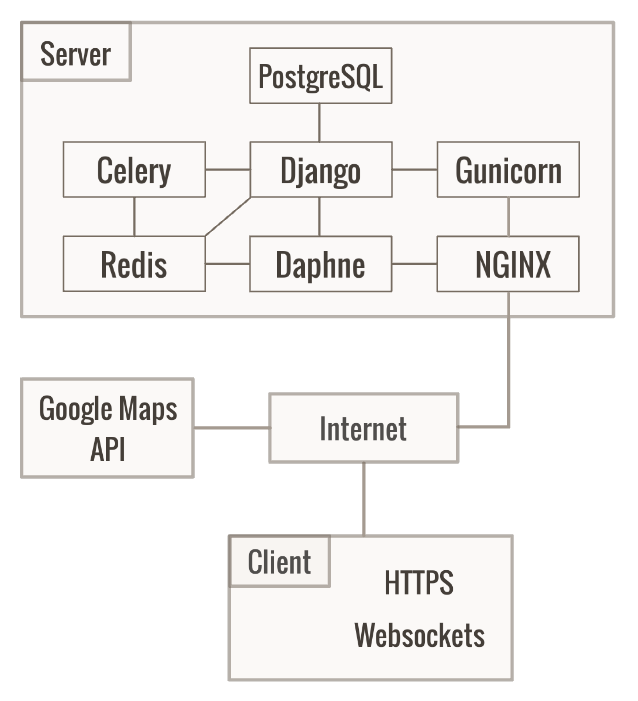
\includegraphics[width=250px]{assets/architecture.png}
\caption{Architecture map for \emph{localhost}}
\label{fig:architecture_map}
\end{figure}

\subsubsection{Execution Path}

When navigating to \emph{localhost}, the client is connected to the NGINX
service. If the required page is a static file such as a CSS or JavaScript
file then the file is immediately served by NGINX. WebSocket requests are
forwarded to the Daphne service (see Section \ref{realtime}). All remaining
requests are forwarded to the Gunicorn web server to then be redirected to
Django.

\subsubsection{Scalability}

The architecture behind \emph{localhost} was designed with scalability as a
priority. The core services on the server are Django and PostgreSQL.
Having multiple other services running concurrently reduces the computation
time available for the core services. While \emph{localhost} was deployed on
a single server, the architecture is designed so that services like NGINX can
be deployed on seperate servers. As NGINX handles the majority of requests
across the web, moving NGINX to a seperate server would significantly improve
the performance of the platform. Each non-core service can have multiple
workers and deployed on multiple servers, ensuring that \emph{localhost} is
scalable.

\subsection{User Interface}
\subsection{Database Design}

\subsection{Real Time Communication}\label{realtime}

The real time communication powering platform features such as notifications,
instant messaging, and bidding events, is provided through the use of web
sockets. WebSockets allow for bi-directional messages to be instantly
communicated with minimal overhead \parencite{websocket}. While Django doesn't
provide support for WebSockets, support can be provided through a third-party
extension for Django called Django Channels.

\subsubsection{MSocket Library \& Django Channels}

Django Channels does not provide native support for multiplex sockets. When
a client application begins listening to an event it must dedicate an entire
socket. Consequently, a client may have multiple sockets open to send and
recieve messages for individual events despite the fact that the traffic could
be sent over a single socket. A server only has a limited number of sockets
available so this reduces the scalability by a significant factor. Multiplex
sockets are sockets that are used to transmit information of different classes
that are then filtered by the reciever and forwarded to the correct recipient
(See Figure \ref{fig:msocket}).

To ensure that \emph{localhost} was scalable, support for multiplex sockets
was provided with a custom client-side JavaScript library and custom Django
class.
\begin{figure}[!h]
  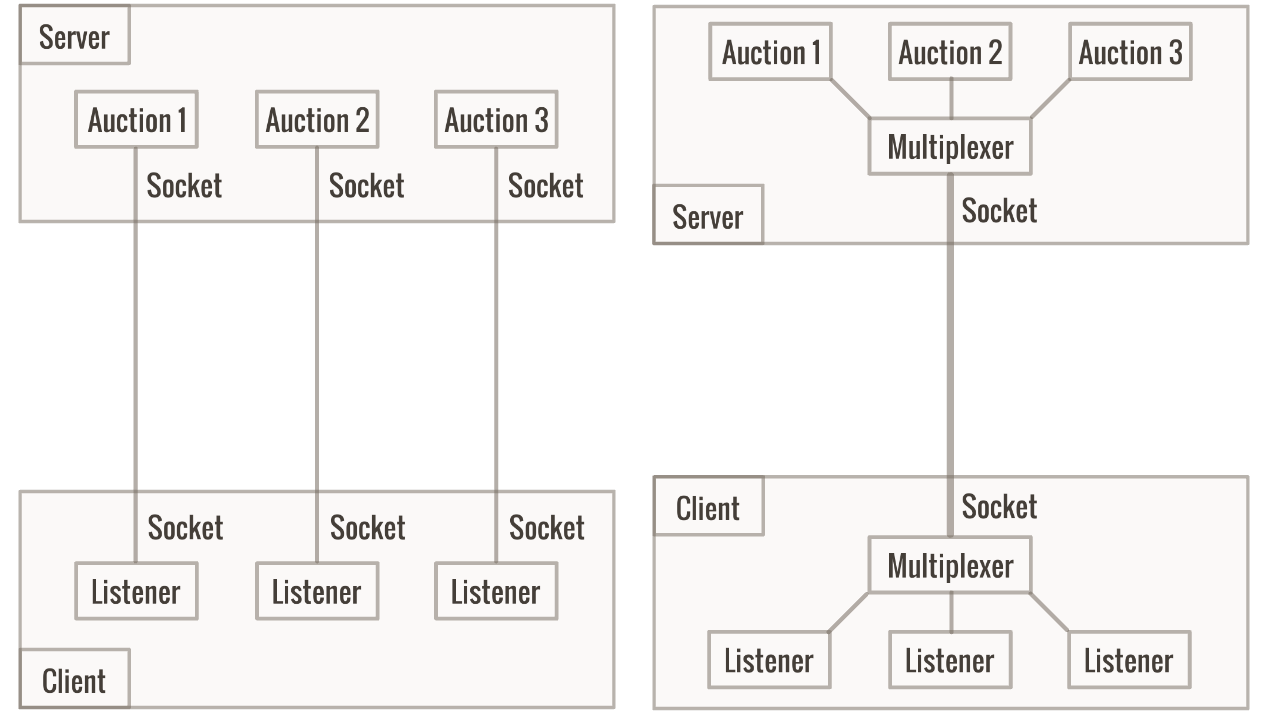
\includegraphics[width=\linewidth]{assets/msocket.png}
  \caption{Comparison between regular sockets and multiplexed sockets}
  \label{fig:msocket}
\end{figure}
The client-side library, called \emph{msocket.js}, is a cooperative multiplex
socket libary. This means that for the socket multiplexing to work, the client
and server must adopt a common protocol of communication. The protocol used
in \emph{localhost} is provided below in the form of a JSON file.
\begin{lstlisting}
{
  type: ,
  data: {

  }
}
\end{lstlisting}

The type allows the multiplexer to determine how to handle the message, and
the data is the payload for the
message. In the case of real-time bidding, the payload would contain details
allowing the handler to determine which property item the bid is for, and how
much the bid is.

\emph{msocket.js} is designed from scratch to provide a simple and abstracted
interface to hide away the details and complexity behind WebSockets. A client
can submit handlers to execute for different types (shown below) and they will
automatically execute as messages of that type arrive.
\begin{lstlisting}
  /**
   * @brief Registers a handler for a message type
   *
   * @param type    The type of message the handler should apply to
   * @param handler The handler to execute on message recieve
   *                Should take the data as an argument
   *                See JSON specification
   *
   * @return On success, @c true
   * @return On failure, @c false when a handler is already set for the type
   * */
  register_handler(type, handler);
\end{lstlisting}

Server-side, the Django Channels socket consumer class was modified to maintain
a record of each of the events the socket is subscribed to and whenever a
message is broadcasted for one of these events the consumer transmits it to
the client with the appropriate class identifier.

\subsection{Event Scheduling}
When an auction session ends, tasks need to be performed in order to complete
the bidding process. There are also several places where scheduled/delayed tasks
are needed in the application.

Property items are said to be ``available'' if the \emph{available} option is
turned on by user (it is ``on'' by default when created) and there are no bids
in all the previous auction sessions in the same day. When the local time
reaches the end time of the session, the system have to check whether there are
bids in the session and create a booking for the winner. Property items that has
been booked out has to be marked as ``unavailable'' so that it does not come up
in the search results. Furthermore, property item has to be re-listed (marked
as ``available'') at 12 noon every day.

\subsubsection{Django Signals}
Signals are dispatched in Django when a certain action is performed within the
framework. It helps decoupled applications to get notified when the actions are
taken placed~\cite{django-signals}. Django provides a set of built-in signals
that allows us to combine it with Celery to perform certain tasks when signals
are dispatched. A list of signals we used in the project are:

\begin{itemize}
  \item \texttt{django.db.models.signals.m2m\_changed}
  \item \texttt{django.db.models.signals.pre\_save}
\end{itemize}

\subsubsection{Celery Beat}
Celery beat is a scheduler in Celery that kicks off tasks at regular intervals,
that are then executed by available worker nodes in the cluster~\cite{celery-beat}.
The worker works asynchronously to start task execution and store results in
a Redis instance.

By default, beat uses \texttt{PersistentScheduler} that keeps track of the last
run in a local shelve\footnote{a persistent, dictionary-like object} database
file. But that is not necessary since we already have a PostgreSQL database
active in the backend. So we instead use an extension
django-celery-beat~\ref{sec:dep-celery-beat} that allows us to store tasks in
the Django database through a \texttt{DatabaseScheduler}. The extension also
provides an admin interface so that tasks could be managed by the administrator.

\paragraph{Periodic Task}
\texttt{PeriodicTask} is a Django model provided by
django-celery-beat~\ref{sec:dep-celery-beat} that simulates how Celery tasks are
represented in the database. We use this in conjunction with
\texttt{DatabaseScheduler} to provide background services in the Django
framework.

\subsubsection{Combining both signals and Celery beat}
There are two tasks to be completed in the background:
\begin{enumerate}
  \item check if anyone bid on a property item; if there is, a booking is added
    to the winner's account, and bids associated with the property item are
    removed. Property item is marked as ``unavailable'' as well. Otherwise we do
    nothing about that property item.
  \item enable bidding for all property items at 12 noon
\end{enumerate}
As such, we define two tasks in Celery accordingly: \texttt{cleanup\_bids} and
\texttt{enable\_bids}. Whenever an auction session is added to a property item
(\texttt{m2m\_changed}), we add a \texttt{PeriodicTask} to the database that
executes \texttt{cleanup\_bids}. A \texttt{PeriodicTask} that executes
\texttt{enable\_bids} is added when a property item is
saved (\texttt{pre\_save}). When celery is launched, the scheduler will pick up
the tasks and triggers tasks execution when time reaches.
